%\documentclass{sig-alternate-10pt}
\documentclass[letterpaper,twocolumn,11pt]{article}
\usepackage{url}
%\usepackage{usenix,epsfig,endnotes}
%\usepackage{fullpage} 
%\setlength{\textwidth}{6.75in}
%\setlength{\oddsidemargin}{-.125in}
\usepackage{graphicx}

\usepackage{natbib}
%\usepackage{subfigure}
%\usepackage{ifpdf}
%\usepackage{multicol}
%\usepackage{amsmath, amssymb, amsthm}
%\usepackage{rotating}
%\onehalfspacing
%\newcommand{\tbd}[1]{[{\bf{#1}}]}

\newcommand{\projectname}[1]{CLINT}
\newcommand{\tbd}[1]{}
\newcommand{\ie}{{\it i.e.}}
\newcommand{\eg}{{\it e.g.}}
\newcommand{\etc}{{\it etc.}}
\newcommand{\apriori}{{\it a priori}}
\newcommand{\eat}[1]{}

\usepackage[usenames,dvipsnames]{color}
\newcommand{\justine}[1]{{\color{ForestGreen}\bf JS: {#1}}}
\newcommand{\andi}[1]{{\color{blue}\bf AW: {#1}}}
\newcommand{\colin}[1]{{\color{Red}\bf CS: {#1}}}

\setlength{\columnsep}{.25in}
\setlength\topmargin{-.5in}
\setlength\textheight{8.5in}
%\usepackage{verbatim}
%\usepackage[compact]{titlesec}
%\usepackage[small]{caption}
\usepackage{times}

% Squeeze out the whitespace!
%\setlength{\parskip}{0pt}
%\setlength{\parsep}{0pt}
%\setlength{\headsep}{0pt}
%\setlength{\topskip}{0pt}
%\setlength{\topmargin}{0pt}
%\setlength{\topsep}{0pt}
%\setlength{\partopsep}{0pt}
%\usepackage[compact]{titlesec}
%\titlespacing{\section}{.5pt}{*.2}{*.2}
%\titlespacing{\subsection}{.5pt}{*.2}{*.2}
%\titlespacing{\subsubsection}{.5pt}{*.2}{*.2}


\title{\vspace{-40pt}\projectname{}: Cross-Layer Debugging for the \\ Software-Defined Networking Stack}

\author{Colin Scott and Justine Sherry\thanks{In collaboration with Andreas
Wundsam, Teemu Koponen, and Scott Shenker}}

%        \begin{multicols}{2}{{\it Draft - Please do not distribute.}}\\
%\author{Paper \#69, 14 Pages}

\date{}
\begin{document}
    \maketitle

\abstract{
{\it
Software bugs are inevitable in software-defined networking (SDN) control planes,
and troubleshooting
is a tedious, time-consuming task.
In this paper we discuss how one might improve
control software troubleshooting by presenting a technique
for automatically identifying
a minimal sequence of inputs responsible for triggering a given bug.
We present three preliminary case studies of real bugs we have found in open source SDN control
platforms---Floodlight, POX, and NOX---and
illustrate how the minimal sequences our technique found were useful for
understanding the root cause of the bugs.

\vspace{45pt}
}

\section{Introduction}
\label{sec:intro}
The SDN platform's $raison\text{ }d'\hat{e}tre$ is to 
hide complexity from control applications. To this end, modern platforms perform
replication, resource arbitration, failure recovery, and network 
virtualization on the control application's behalf. 

While these measures are effective in simplifying control applications,
they do not remove any complexity from the overall system. Rather, they merely move the complexity
from control applications into the underlying SDN platform.

As in any software system, additional complexity increases the probability of
bugs. And unfortunately for the network operator, finding bugs in the platform requires
access to precisely the details hidden from the control application.
When operators encounters erratic behavior in their network, the error's root
cause may lie in their own policy specification, or in the SDN platform
itself. To deal with the latter case, they must trace through
multiple layers of abstraction: virtualization logic, distribution logic, and
network devices.

As it stands, the SDN platform provides meager support for troubleshooting.
The predominant troubleshooting method is log analysis: manually
specifying log statements at relevant points throughout the system,
collecting; gathering; and ordering distributed log files; and analyzing the
results {\it post-hoc} when a error is encountered in production. Besides its
apparent tediousness, this approach is lacking in several ways: logs events
are enormous in number, impossible to aggregate into a single serial
execution of the system, and often at the wrong level of granularity to be of
use.

Recent work has contributed much-needed improvements to the highest (control
application) and lowest (dataplane forwarding tables) levels of abstraction, 
but no principled troubleshooting mechanism exists yet for the SDN platform.
NICE applies concolic execution and model checking to SDN control
applications, thereby automating the testing process and catching bugs before
they are deployed~\cite{nice}. Aneater~\cite{anteater} and HSA~\cite{hsa}
introduce mechanisms for checking static invariants in the dataplane.

It would be unthinkable to introduce a new programming language without a
debugger. Similarly, we think it highly undesirable to deploy SDN-based
networking without a viable troubleshooting paradigm. 

Correctness of the SDN platform can be stated concisely: high-level policies
should correspond with low-level configuration. We observe that the structure
of the SDN platform, graphs at every layer, enables a straightforward
algorithm to check this invariant. Our algorithm, which we term correspondence checking,
enumerates all inconsistencies at any point in time and isolates the
root cause of an inconsistency to a particular component of the system.

In eventually-consistent systems such as software-defined
networks however, transient inconsistencies between network policy and actual network
behavior are an inevitable state-of-affairs.
In such an environment, it does not suffice for troubleshooting tools to
simply enumerate inconsistencies; they should also aid the developer
in identifying which are related to serious problems, and which are
harmlessly ephemeral. To this end we present \simulator.
\Simulator allows troubleshooters 
to sift out pernicious inconsistencies by tracking the life cycle of problems 
both forward and backward in time.

We have implemented prototypes
of correspondence checking and \simulator. Our code is publicly available
at~\cite{github}.

The rest of this paper is organized as follows. In \S\ref{sec:overview},
we present an overview of the SDN stack and its failure modes.
In \S\ref{sec:approach} we present correspondence checking and
\simulator in detail. In \S\ref{sec:evaluation} we present
two use-cases and a preliminary performance evaluation
Finally, in \S\ref{sec:related_work} we discuss related work,
and in \S\ref{sec:conclusion} we conclude.


\section{SDN Failure Modes}
\label{sec:bug_analysis}

In this section we provide an analysis of the classes of errors observed in
production-grade software-defined networks. We base our analysis on conversations with
researchers at Nicira~\cite{nicira}, a startup focused on developing a network operating
system for production SDN deployments~\cite{onix}.

\begin{figure}[t]
    \centering
    \begin{tabular}{ccc}
    \hspace{-5pt}\includegraphics[width=.9in]{../diagrams/bugs/loop.pdf}&
    \includegraphics[width=.9in]{../diagrams/bugs/dead_end.pdf}&
    \includegraphics[width=.9in]{../diagrams/bugs/partition.pdf}\\
    {\bf (i) Loop}&{\bf (ii) Black Hole}&{\bf (iii) Partition}\\
    \end{tabular}
    \caption[]{\label{fig:invariantviolations} Selected classes of physical network errors detectable with static
    checking.\vspace{-10pt}} 
\end{figure}

\colin{Insert diagrams on bugs that we can catch but Anteater can't}

What kind of bugs do we want to analyze? Well I guess we start with static
bugs that Anteater can detect. Useful for providing background common error
conditions seen in networks. 

Well, loops are these things where packets go in a circle and never come out.
Their bad because they cause the traffic stuck in the loop to never go
through. They're also bad because they congest the routers in the loop, and
therefore affect unrelated traffic. Really bad at layer 2, where there are no
ttls.

Ok. Then there are partitions. In most cases, every host in the network should
be able to reach every other host in the network. If there exists no route to
one host, 

Blackholes are a related problem. Traffic may arrive at a dead end,

Maybe talk about routing consistency? Simplest invariant is `No packet can
arrive at a web server without passing through a firewall`. If re-distributing
load across ingress switches, in-flight packets might get the web server
without passing through a firewall.

Ok, now for the interesting bugs. Start with Justine's flow overlap bug.

Then go on to virtualization bugs. These are pretty severe, by the way.
Semantic mismatches, yahdah yahdah.

Then consistency. 9 in 10 systems researchers agree, PAXOS is hard.



\section{Approach}
\label{sec:approach}
We have developed a technique, \simulator, for automatically identifying
a minimal sequence of inputs responsibly for triggering a given
bug. Here we detail the specifics
of \simulator.

We start by describing an example bug in the Floodlight
open source control platform~\cite{floodlight_bug} to illustrate the mechanics
of our technique. Floodlight is distributed across
multiple controllers for high availability, and provides support for
virtualization. Switches maintain one hot connection to a master controller and
several cold connections to replica controllers. The \emph{master} holds the
authority to modify the configuration of switches, while the other
controllers are in \emph{backup} mode and do not perform any changes to the
switch configurations unless they detect that the master has crashed.

\begin{figure}[t]
    %\hspace{-10pt}
    \includegraphics[width=3.25in]{../diagrams/case_study/example_bug.pdf}
    \caption[]{\label{fig:example} Floodlight failover bug. External inputs
               are depicted as red dots, internal events are depicted as black
               dots, and the dotted messages line depicts a timeout.}
\end{figure}

The failover logic in Floodlight is not implemented correctly, leading to the
following race condition\footnote{Note that this issue was
originally documented by the developers of Floodlight~\cite{floodlight_bug}} depicted in
Figure~\ref{fig:example}:
a link fails (E1), and the switch attempts to notify the controllers (E2,E4) shortly after the master
controller has died (E3), but before a new master has been selected (E6). In this case, all live controllers are in
the backup role and will not take responsibility for updating the switch
flow table (E5). At some point, a backup notices the master failure and
elevates itself to the master role (E6). The new master will proceed to manage
the switch, but without ever clearing the routing entries for
the failed link (resulting in a persistent blackhole).

There were only two external inputs (E1,E3) shown in our example.
Even relatively simple cases may contain extraneous inputs, making it difficult
for a troubleshooter to reason about the underlying root cause.
In the worst case, operators may need to examine logs from a production
network, which contain a substantial number of hardware failures, topology changes,
and other potential triggering events,
all of which may appear characteristic of normal operating
conditions at first glance; assuming 8.5 network error events per
minute~\cite{Greenberg:2009:VSF:1592568.1592576}, 500 VM migrations per
hour~\cite{Soundararajan:2010:CBS:1899928.1899941}, and a relevant execution
history of one hour, there would be over 1000 inputs to the system
reflected in the log.

Given a trace of the system execution similar to the Floodlight case,
our goal is to prune events that are not
necessary for triggering errant behavior. We define errant behavior in terms
of {\em correctness violations}:
configurations of the network that are inconsistent
with the policy. In the example, the correctness violation is between a
reachability policy specified in the logical view (``A can talk to B'')
and the blackhole in the physical network (``A's packets to B enter the
blackhole and do not arrive at B'').

We have developed a technique to automatically perform this pruning.
Specifically, our technique identifies a minimal sequence of inputs
to the controllers that is sufficient for triggering a known correctness violation. We
refer to such inputs as a {\em minimal causal sequence} (MCS). Going back to our example,
suppose the log includes many more (extraneous) inputs. Whenever an
extraneous event is pruned, the blackhole will still persist. When
the controller crash is pruned, the blackhole will be resolved properly, and
when the link failure is pruned, no blackhole will occur. The MCS returned
is therefore the controller crash and the link failure in conjunction.

\subsection{Delta Debugging}
\label{subsec:algorithm}

Delta debugging~\cite{Zeller:2002:SIF:506201.506206}, a technique from the
software engineering community, gets us part of the way
there: given a single input (\eg~an HTML page)
for a non-distributed program (\eg~Firefox), it performs a divide-and-conquer
search, repeatedly running the program on subsets of the input
until it finds a minimal subset (\eg~a single tag) that is sufficient
for triggering a known bug. The delta debugging algorithm is shown in
Figure~\ref{fig:ddmin}.

\begin{figure*}[t]
\caption{Minimizing Delta Debugging Algorithm From~\cite{Zeller:2002:SIF:506201.506206}}
\begin{boxedminipage}{\textwidth}
Input: $\cfail$ s.t. $\cfail$ is a trace and $\test(\cfail) = \FAIL$. Output: $\dfail
= \ddmin(\cfail)$ s.t. $\dfail \subseteq
\cfail$, $\test(\dfail) = \FAIL$, and~$\dfail$ is 1-minimal.
\begin{align*}
\ddmin(\cfail) &= \ddmin_2(\cfail, 2) \quad \text{where} \\
\ddmin_2(\dfail, n) &= 
\begin{cases}
\ddmin_2(\Delta_i, 2) & \text{\hphantom{else }if $\exists i \in \{1, \dots, n\} \cdot \test(\Delta_i) = \FAIL$ (``reduce to subset'')} \\
\ddmin_2\bigl(\nabla_i, \max(n - 1, 2)\bigr) & 
\text{else if $\exists i \in \{1, \dots, n\} \cdot \test(\nabla_i) = \FAIL$ (``reduce to complement'')} \\
\ddmin_2\bigl(\dfail, \min(|\dfail|, 2n)\bigr) & \text{else if $n < |\dfail|$ (``increase granularity'')} \\
\dfail & \text{otherwise (``done'').}
\end{cases}
\end{align*}
where $\test(T)$ denotes the state of the system after executing the trace $T$,
$\FAIL$ denotes a correctness violation, \\
$\nabla_i = \dfail - \Delta_i$, $\dfail = \Delta_1 \cup \Delta_2 \cup \dots \cup \Delta_n$, all
$\Delta_i$ are pairwise disjoint sequences of inputs, and $\forall \Delta_i \cdot |\Delta_i| \approx |\dfail| / n$
holds.
\end{boxedminipage}
\label{fig:ddmin}
\end{figure*}

Our problem differs from the original formulation of delta debugging in two dimensions.
First, input to SDN controllers is spread
across time: it includes many messages, and depends on subtle causal
relationships. Second, the input is spread across space: it involves
many concurrently running nodes.
In the rest of this section, we describe how we
replay inputs to control software,
cope with alterations to the causal history of an execution, and check
for correctness violations. In \S\ref{sec:architecture}, we describe concrete
ways \simulator~can be put to use.

\subsection{Simulation}
\label{subsec:simulation}

Unlike the example applications described
by Zeller et al.~\cite{Zeller:2002:SIF:506201.506206}, the system we are troubleshooting is not a
single program--it is all the nodes and links of a distributed system,
including controllers, switches, and end-hosts. Replaying traces
on an actual network would be prohibitively costly and overly prone to
non-deterministic behavior. We therefore simulate the entire control-plane,
with support for minimal data-plane behavior,
in a single process. We then run the control software on
top of this simulator and connect the software switches to the controllers as if they were true
network devices, such that the controllers believe they are configuring a true
network. This setup allows the simulator to interpose on all communication
channels, enabling fine-grained control over message orderings. The overall
simulation architecture is depicted in
Figure~\ref{fig:architecture}.

\begin{figure}[t]
    %\hspace{-10pt}
    \includegraphics[width=3.25in]{../diagrams/architecture/Debugger_Architecture.pdf}
    \caption[]{\label{fig:architecture} Simulation infrastructure. Dataplane
    devices run in software, and all communication channels are
    interposed upon.}
\end{figure}

Given a sequence of inputs (\eg~link failures, controller crashes, host migrations,
or policy changes) and an invariant checking probe (provided by frameworks
such as HSA~\cite{hsa,hsa_realtime} or Anteater~\cite{anteater,khurshid2012veriflow}), the simulator invokes
the delta debugging algorithm to identify the minimal causal set. The
simulator is then responsible for replaying intermediate input subsequences
chosen by delta debugging. For example, link failures are
reproduced by disconnecting the edge in the simulated network, and sending a
port status message from the adjacent switches to their parent controller(s).

\subsection{Replay}
\label{subsec:replay}

The timing of the inputs injected by the simulator is crucial for ensuring that the
execution is the same as the original run. Na\"ively injecting inputs often fails to
trigger the original correctness violation, even without having pruned any
events. In particular, we tried and failed to reproduce errors when scheduling inputs
with the following simple algorithm:
\begin{align*}
t'_0 = 0 \\
t'_i = t'_{i-1} + |t_{i} - t_{i-1}|
\end{align*}
where $t'_i$ is the simulation's clock value when it injects the $i^{th}$ input, and $t_i$ is
the timestamp of the $i^{th}$ input from the original run. In other words, simply
maintaining the relative timing between inputs is not sufficient.

The problem with the simple scheduling algorithm is that it does not take into
account events that are internal to the control software, such as
message receipts, timers going off, or internal state
changes like the backup node in the Floodlight example deciding to elevate itself to master.
Consider for example that if a controller's garbage collector happens to run
while we replay inputs, it is feasible that the delicate ordering between
inputs internal events would be perturbed, resulting in a different output.

Formally, we need to inject an external input $e$ at exactly the point when all other
events (both external and internal) that precede it in the happens-before
relation ($\{i \mid i \rightarrow e\}$) from the original execution have occurred.
While the input and internal events from the original run are given to us,
we become aware of internal events throughout replay by
(i) monitoring
control message receipts between controllers and between switches and
controllers, and (ii) interposing on the controllers' logging library and notifying the
simulation process whenever log statement (which serve to mark relevant state
transitions) is executed. Note that to achieve truly deterministic
replay, these log statements would need to
be highly granular, capturing information such as thread scheduling decisions;
we show in \S\ref{subsec:case_studies}
however that pre-existing, course granular log statements are sufficient to
successfully reproduce many bugs.\footnote{We discuss this problem further in \S\ref{subsec:domain_knowledge}}
%Note that the developer must provide enough logging statements
%so that relevant internal state changes are captured and visible to our
%tool.

\subsection{Fingerprinting}
\label{subsec:fingerprinting}

Event scheduling is made substantially more complicated by the fact
that the delta debugging algorithm is pruning inputs from the history of the
execution, thereby changing the resulting internal events generated by the control
software. One implication of this is that the syntax of the internal events may differ
slightly from their equivalent internal events in the original
execution. Consider for example that sequence numbers of control packets may
all differ by one if a single control message in the beginning of the trace
does not occur.

Our solution is to define domain-specific masks over
semantically extraneous\footnote{*Extraneous with respect to comparing two
separate traces. For example, the buffer id is chosen at random, so
it is meaningless to compare buffer ids across separate runs. One consequence
of masks is that bugs involving masked fields are outside the purview of
\simulator.} fields of
the message. A few examples of masked fields are shown
in Table~\ref{tab:fingerprints}. These masks define equivalence classes
of internal events, which allow us to compare different runs of the simulation.
Formally, we consider an internal event $i'$ observed in an altered trace
equivalent to an internal event $i$ from the original trace iff all unmasked
fields have the same value
and $i$ occurs between $i'$'s preceding and succeeding inputs in the
happens-before relation.

\begin{figure}[t]
    %\hspace{-10pt}
    \includegraphics[width=3.25in]{../diagrams/state_machines/controller_switch.pdf}
    \caption[]{\label{fig:state_machines} Simplified state machines for the switch and
    controllers in the example Floodlight bug. Double outlined states
    represent presence of the blackhole.}
\end{figure}

\begin{table}
\centering
\begin{tabular}{|l|l|}
\hline
Internal message & Masked values \\
\hline
OpenFlow headers & transaction id\\
OpenFlow FLOW\_MODs & cookie, buffer id \\
Log statements & varargs parameters to printf \\
\hline
\end{tabular}
\caption{Example internal messages and their masked values. The masks serve to
define equivalence classes.}
\label{tab:fingerprints}
\end{table}

\subsection{Coping With Divergence}
\label{subsec:divergence}

A deeper implication of altering the original trace is that
some internal events from the original run may not occur after
pruning certain inputs--conversely, new internal events not present in the original run
may occur. Consider the simplified state machines for the switch and
controllers from the Floodlight case shown in
Figure~\ref{fig:state_machines}. If link failure input is pruned, the
switch will not make the transition to `Notify Parents', and the master will
consequently not make the transition to and from `Send Flush'. Without being
able to equate events from alternate histories, it is nearly impossible to resolve
divergences like this in a way that ensures that the original bug is still
triggered.

We have developed two event scheduling algorithms to account for altered
internal events. The first is simpler, but somewhat less robust. We refer to it as
\emph{waiting replay}, and it is shown in Figure~\ref{fig:simple_algorithm}.
Simply put, it waits for internal events matching those in the original run,
but times out and proceeds if they do not occur.

\begin{figure}
\begin{boxedminipage}{\linewidth}
\begin{Verbatim}[commandchars=\\\{\}]
for e\textsubscript{i} in trace:
  if e\textsubscript{i} is an internal event:
    \textDelta = |e\textsubscript{i}.time - e\textsubscript{i-1}.time| + \textepsilon
    wait up to \textDelta seconds for e\textsubscript{i}
  else: // input
    inject e\textsubscript{i}
\end{Verbatim}
\end{boxedminipage}
\caption{Waiting Replay Algorithm}
\label{fig:simple_algorithm}
\end{figure}

In most cases waiting replay successfully reproduces the original correctness
violation, assuming \textepsilon~is larger than variations in execution speeds
between internal events. If the value of \textepsilon~is too large, however, we may end up
waiting too long for the happens-before predecessors of an input $e_i$ such that a
successor of $e_i$ occurs before we have injected $e_i$,
potentially resulting in an altered output.
% \sam{Is it worth noting that this isn't necessarily a problem? If a successor occurs, it means it wasn't causally related to $e_i$, but the ordering still might matter for further successors.}

Our second event scheduling algorithm addresses this possibility, but
adds a factor of $n$ in the number of replayed inputs to the overall
runtime. We refer to it as \emph{peeking replay}, and it is shown in Figure~\ref{fig:peek}.
Simply put, peeking replay
attempts to precompute which internal events are and aren't going to occur
between any adjacent pair of inputs
so that it can know exactly how long to wait before injecting inputs in the
final replay.

\begin{figure}
\begin{boxedminipage}{\linewidth}
\begin{Verbatim}[commandchars=\\\{\}]
inputs = [e\textsubscript{1}, e\textsubscript{2}, ..., e\textsubscript{n}]
new\_trace = []

for i in 1 to n-1:
  waiting\_replay(new\_trace + [e\textsubscript{i}], \textepsilon=0)
  start recording internal events
  \textDelta = |e\textsubscript{i+1}.time - e\textsubscript{i}.time| + \textepsilon
  wait \textDelta seconds
  remove successors of e\textsubscript{i} from \textbackslash
    recorded internal events
  new\_trace += [e\textsubscript{i}]
  new\_trace += recorded internal events

waiting\_replay(new\_trace + [e\textsubscript{n}], \textepsilon=0)
\end{Verbatim}
\end{boxedminipage}
\caption{Peeking Replay Algorithm}
\label{fig:peek}
\end{figure}

% TODO: not quite true!
In practice we employ a hybrid algorithm
that defaults to waiting replay and only
peeks during intervals where it has waited too long.
This is possible because waiting replay can always detect when it has
waited too long upon observing a successor of the input to be injected.
Although the hybrid algorithm has the same worst case runtime as peeking
replay, the average case runtime is significantly better.

Waiting and peeking replay both need to account for the pathological case
where {\em multiple} internal events in the same
equivalence class a single internal event in the original execution.
Ambiguous equivalences mean that more than one possibility exists for where
the next input should be
injected while still maintaining happens-before constraints. For example, if $i_2$ and $i_3$ are internal events observed
during replay that are both in the same equivalence class as a single event $i_1$ from the
original run, one might inject the next input after $i_2$ or after $i_3$.
As we have proven elsewhere,\footnote{URL omitted for anonymity reasons}
all possibilities need to be explored to guarantee that if a path through the
distributed state machine leading to
the correctness violation from the original execution exists, that path will be taken. In the worst case,
this implies an exponential number of possibilities to be explored during
replay.

Luckily, ambiguous equivalent internal events are extremely rare in the
control software we evaluated, as we
show in \S\ref{subsec:runtime}. We have proven elsewhere that ambiguity only
occurs when a sub-path exists in the distributed state machine that contains two or
more equivalent internal edges without an intermediate input event edge.
We conjecture that such transitions are not common in control plane systems,
which are designed to quiesce quickly (\ie~take a small number of internal
transitions after any input event). Consider the state machines in Figure~\ref{fig:state_machines}:
it is not possible to traverse the same internal event edge (``Receive Link
Failure Notification'' or ``Receive Flush'') without traversing an
intermediate input event edge (``Link Failure'' or ``Master Failure'').
\colin{TODO: need a figure that shows generalized event scheduling}

\subsection{Complexity}
\label{subsec:complexity}

Assuming no ambiguities occur, the delta debugging algorithm terminates after
$O(log\,n)$
invocations of $replay$ in the best case, where $n$ is the number of inputs in the original
trace~\cite{Zeller:2002:SIF:506201.506206}. Each invocation of waiting replay
injects $n$ inputs, for an overall runtime of $O(nlog\,n)$ for
waiting replay. The worst case runtime of delta debugging is $O(n^2)$ in the
number of invocations of $replay$~\cite{Zeller:2002:SIF:506201.506206}.
Therefore the overall worst case runtime is $O(n^3)$ if waiting replay is used.

Peeking replay adds another factor of $n$ to the overall runtime: for each input event
$e_i$, it invokes waiting replay with inputs $e_1,\dots,e_i$, for a total of
$n \times \frac{n+1}{2} \in O(n^2)$ replayed inputs. Therefore in the
best case, the overall runtime of delta debugging with peeking replay is
$O(n^2log\,n)$, and the worst case is $O(n^4)$. Note that this extra factor of
$n$ in computational complexity can be converted to a factor of $n$ in storage
complexity if peek stores snapshots of
the controllers' state rather than replaying each prefix from the beginning.

\subsection{Parameters}
\label{subsec:params}

Both waiting and peeking replay leave an open question as to what value
\textepsilon~should be set to. In our current implementation,
we set \textepsilon~somewhat
arbitrarily to $100$ milliseconds, and this has worked for \num{most} of our
failure cases. In general, larger values of \textepsilon~are preferable to
smaller values (disregarding runtime considerations), since we can always
detect when we have waited too long (\viz~when a successor of the next input
has occurred), but we cannot detect when we have timed out
early on an internal event that is in fact going to occur.

In practice we also make optimization to the overall delta debugging
algorithm: since some of the input subsequences
chosen by unmodified delta debugging may not be valid, we apply domain knowledge
about input validity to avoid exploring certain subsequences. For example, it does
not make sense to replay a link recovery event if we pruned
the link failure event that preceded it. Likewise, pruning a host migration
implies that we need to update the subsequent host migration event's source location.
Beyond component failures and host migration, other dependencies between
inputs are significantly more complicated to model.
%At the
%moment, our tool does not support policy changes or dataplane packet drops for
%this reason.

\colin{Mention that causal
annotations and selective pruning help.} \colin{Make sure we emphasize that there is no `right answer', since we're
dealing with modified histories}.

\subsection{Correspondence Checking}
\label{subsec:cc}

\num{Cut if no space.}
Finally, we need a mechanism for deciding
whether a correctness violation is present at the end of the system execution.
We refer to such an algorithm as a {\em decider}.

\Simulator~supports generic deciders (\eg~all-pairs reachability or loop detection),
provided by frameworks such as Hassel~\cite{hsa,hsa_realtime} or
Anteater~\cite{anteater,khurshid2012veriflow}.
With a small modification to the control software however, we can
extract the network policies already reflected in the
controller's data structures and thereby check a much more fine-grained set of invariants.
We refer to this technique as correspondence checking. Correspondence checking
builds on the virtual packet algebra
pioneered in headerspace analysis~\cite{hsa}.

Formally, the state of the physical network, the physical view (the
data structure maintained by the controllers for tracking the current state of the physical
network), and the
logical view (the data structure maintained by the controllers for storing
network policies in a routing table-like format) can be represented as graphs,
$G = (V, E)$. Packets are series of bits, $h \in \{0,1\}^L$ in the universe
of all possible bit sequences $H = \{0,1\}^L$,
where $L$ is the maximum number of bits in the header.

Upon receiving a packet,
forwarding elements apply a transformation function, potentially modifying
packets before forwarding them on\footnote{Multicast forwarding can expressed
by extending the range to sets of output tuples}:
\begin{align*}
T: (H \times E) \rightarrow (H \times E_{\emptyset})
\end{align*}
Here, $E_{\emptyset} \equiv E \cup \emptyset$, signifying that forwarding elements
may drop packets.

We use $\Psi$ to denote the collection of all transfer functions present in
the network at a particular point in time. In this model, network traversal is
simply repeated application of $\Psi$.
For example, if a header $h$ enters the network through edge
$e$, its state after $k$ hops will be:
\begin{align*}
\Psi^k(h,e) = \Psi(\Psi(\dots \Psi(h,e)\dots))
\end{align*}

The externally visible behavior of the network can be expressed as the
transitive closure of $\Psi$:
\begin{align*}
\Omega: (H \times E_{access}) \rightarrow (H \times E_{\emptyset}) \\
\Omega(h,e) = \Psi^{\infty}(h,e)
\end{align*}
Here, $E_{access}$ denotes access links adjacent to end-hosts.

The domain of $\Omega^{physical}$ is the set of pairs of end-hosts in the
physical network along with packets they could possibly produce (before
the packets have been encapsulated). We define $\Omega^{view}$ in exactly the same way, where
the logical hosts are abstract representations of the hosts in the physical
network. This definition depends on the observation that end-hosts are represented
in all layers, even if there is not a one-to-one mapping between the
internal vertices of $G^{virtual}$ and $G^{physical}$.

The range of $\Omega$ is the hypothetical final state of the
input packet if it were injected in the network.
We use the special value $LOOP$ to distinguish
a packet dropped by a network device from a packet entering an
infinite loop (both of which never leave the network).

In SDN, it should always be the case that:
\begin{align*}
\Omega^{view} \sim \Omega^{physical}
\end{align*}
The equivalence $\sim$ means that the final outcome of any input packet
injected at a host $a_{physical}$ in the physical network has the same hypothetical final outcome as
the same input injected at the corresponding $a_{logical}$, and vice versa.

Correspondence checking takes as input a
snapshot of both the physical network and the
controllers' state. We first modify the control software to present an
interface through which the physical and virtual views can be
extracted. The snapshot is
then obtained by pausing execution and invoking this interface.
The routing tables of forwarding elements in the views and the physical
network can then be translated into transformation functions.
Finally, we feed a symbolic packet $x^L$ to each access link of the
network.\footnote{The rules for process wildcard bits $x^n$ are defined in
the HSA paper~\cite{hsa}} The end result is a propagation graph representing
all possible paths taken by any packet injected
at the access link.

We compute $\Omega$ by traversing the resulting propagation graph. If a packet
enters a loop before exiting the network, we mark the value as
$LOOP$. Otherwise,
the leaves of the propagation graph define the final outcomes of the input
packets injected at that access link. Because network policies are defined by
configuring the logical view, any mismatch between $\Omega^{view}$ and $\Omega^{physical}$
represents an instance of a correctness violation. Note that mismatches are
unambiguous; that is, two slightly different correctness violation from
different runs of the system are always distinguishable.

Note the price of correspondence checking's generality is that it represents
a somewhat weak notion of
correctness. Correspondence checking only captures external behavior and
loops; it does not capture internal behavior such as load-balancing
over links. It also assumes that the policies as expressed by the
configuration of the logical view are correct. Finally, correspondence
checking can not verify
time-dependent policies such as ``No link should be congested more than 1\% of
the time''.

\subsection{Limitations}
\label{subsec:non_goals}

Having detailed the specifics of \simulator, we now
clarify the scope of its technique's use.

\noindent{\bf Troubleshooting vs Debugging.} Our technique is a troubleshooting tool, not a debugger;
by this we mean that \simulator{} helps identify and localize inputs that
trigger erroneous behavior, but it does not directly identify which
line(s) of code cause the error.

\noindent{\bf Bugs Outside the Control Software.} Our goal is not to find the root
cause of individual component failures in the system (\eg~misbehaving routers,
link failures). Instead, we focus on
how the distributed system as a whole reacts to the occurrence of inputs such
as component failures.
If there is a bug in your switch, you need to contact your hardware vendor;
if you have a bug in your policy specification, you need to take a closer look at what you specified.
That said, our tool can show whether switches behave the same as our software
implementation: if our tool was unable to reproduce the error, that means that
the problem was above or below the control software.

\noindent{\bf Non-determinism Within Individual Controllers.} Our tool is not designed to reproduce bugs
involving non-determinism within a single controller (\eg~race-conditions between threads);
we focus on coarser granularity errors (\eg~incorrect failover logic), which we find plenty of
in \S\ref{subsec:case_studies}. The upshot of
this is that our technique is not able to minimize all possible failures, such as
data races between threads.
Nonetheless, the worst case for us is that the developer ends up with what they started:
an unpruned log. That said, if the developer is willing to instrument their system to
provide finer granularity log messages (\cf~\cite{Geels:2006:RDD:1267359.1267386}),
our approach readily supports deterministic replay.

\noindent{\bf Globally vs Locally Minimal Input Sequences.}
Our approach is not guaranteed to find the globally minimal
causal sequence from an input trace, since this requires $O(2^N)$ computation in the worst case.
The delta debugging algorithm we employ however is guaranteed to find a 1-minimal
(locally minimal) causal sequence~\cite{Zeller:2002:SIF:506201.506206},
meaning that if any input from the sequence is pruned, no correctness violation
occurs.

\noindent{\bf Correctness vs Performance.}
We are primarily focused on correctness bugs, not performance bugs. That said,
our approach is largely agnostic to what invariants are
checked.

\noindent{\bf Proactive vs Reactive Configuration.} We focus primarily on
\emph{proactive} configuration, where controllers react to policy and topology changes, but
not necessarily individual packets or flows events in the
dataplane.\footnote{Production controllers typically adopt this model for performance reasons}
The main challenge in extending our approach to reactive controllers is
achieving efficient simulation of dataplane traffic.

% ---------------------------------------------- %
%             OLD TEXT
\eat{

%Platform developers may discover correctness violations
%through customer complaints, integration tests, or by periodically running
%invariant checks on a deployed network.

\subsection{\SIMULATOR{}}
\label{sec:causal_analysis}

We have developed an algorithm, \simulator{}, for automatically inferring the inputs to the
controllers that are both necessary and sufficient for triggering the correctness violation. We
refer to these events as the {\em minimal causal sequence} (MCS). We show
the algorithm here, and elaborate in later sections:

\begin{Verbatim}[commandchars=\\\{\}]
Input: E = [e\textsubscript{1}, e\textsubscript{2}, e\textsubscript{3}, e\textsubscript{4}, ... e\textsubscript{n}]
Output: MCS

MCS = []
for i in 1 to n:
  if violation in replay(E - e\textsubscript{i}):
    E := E - e\textsubscript{i}
  else:
    MCS := MCS || e\textsubscript{i}
\end{Verbatim}

\noindent In words, the algorithm takes in a log of the system execution,
prunes each external input in isolation,
runs the system forward with the remaining input, checks whether the
correctness violation is still present, and thereby infers whether that input is
necessary for triggering the fault. Going back to our example, suppose the
log includes many more (extraneous) inputs. Whenever an
extraneous event is pruned, the blackhole will still persist. When
the controller crash is pruned, the blackhole will be resolved properly, and
when the link failure is pruned, no blackhole will occur. The MCS returned
is therefore the controller crash and the link failure in conjunction.

The crux of our contribution lies in specifying exactly how each
individual step of this algorithm works. In the rest of this section we will
describe our efforts to support \simulator{}, including (i)
detailing how execution logs are obtained
and what properties they need, (ii) developing a deterministic network simulator
to replay the execution of control software, and (iii) developing an invariant
checking algorithm for detecting errant behavior.

\subsection{Distributed Logging}

\Simulator{} first requires a log of the system execution where a
correctness violation was originally discovered. Correctness violations
in a running system might be detected through failed integration tests,
customer complaints, or online invariant checks. \colin{Use the word
``Forensically''}

Since our goal is to identify
relevant {\em inputs} from the distributed system's log, the log must make a clear
distinction between {\em internal} events such as control message sends and
receives, and {\em external} inputs such as
link failures, controller crashes, VM migrations, or policy changes.
Production networks almost universally maintain logs of such events as part of
good operating practices (link failures are typically detected through
protocols such as IS-IS,
controllers log crash messages before
halting in addition to monitoring heartbeats from peers, and VM migrations and
policy changes are logged centrally for accounting purposes). In
\S\ref{sec:discussion} we discuss the size of these logs, and truncation that can be
performed.

\Simulator{} also depends on a causally ordered log of the
distributed system's execution. Most production systems already maintain a
total ordering with clock synchronization (e.g. NTP) or Lamport clocks. If the control software does not already do
so, we modify the code to attach Lamport
clocks to all
control packets and internal log messages
to achieve a total ordering of the events in the system that
is consistent with the happens-before
relation~\cite{Lamport:1978:TCO:359545.359563}.

\eat{
As an optimization, the developer may start from a causally-consistent
snapshot of the network rather than replaying the execution from the
very beginning of the log. In this case, the user would need to occasionally
execute a consistent-snapshotting algorithm~\cite{Chandy:1985:DSD:214451.214456}
on the live deployed system, and start \simulator{} from a quiescent snapshot.
}

%(ii) We assume that the causally-consistent snapshot we start from is quiescent. [it's possible that a member of the MCS occurred before the snapshot was taken]
%
%Solution/Workaround: once we've run the MCS algorithm, re-run it from an earlier snapshot and see if the MCS changed. Technically this process would have to be applied inductively, but we could parameterize the number snapshots we have to examine.
%
%Discussion: it's also not a huge deal if this assumption does not hold. The correctness violation will still be detected -- the only problem is that the MCS will be smaller than it actually is. Moreover, as the software developer starts debugging the problem, she'll eventually notice that some piece of state at the point of the snapshot is incorrect, and therefore she'll notice that she needs to start from an earlier snapshot.

\eat{
\colin{In the simulator, this consistent snapshot is
trivial to take: simply pause each controller's VM and the simulation. To
obtain the snapshot that denotes time zero, we assume that the production
network takes periodic snapshots using an algorithm such as Chandy et al's
\cite{Chandy:1985:DSD:214451.214456} consistent snapshot algorithm}
}

\eat{
{\em Causally-consistent snapshot:} a snapshot of a distributed system's state where
there exists no event $b$ in a node's event history such that $a \rightarrow
b$, but $a$ does not appear in the snapshot.
}

\eat{
{\em External events:} input fed to the control platform triggered by processes outside
of the system. For proactive controllers, external input includes policy
changes, host placement changes, network topology changes (including hardware
failures), and control server failures. Reactive controllers
additionally take traffic changes as input. External events are to be distinguished
from internal events triggered by the system itself, such as message sends or software
crashes.
}

\subsection{Deterministic Replay}

Next, \simulator{} requires the ability to replay the system execution.
We have developed solutions to two separate challenges in achieving this requirement.

First, the system replay has to be {\em deterministic}.
We achieve this by simulating the entire network, including hosts and
switches, in a single-threaded process, and running the controllers in
individual virtual machines that are
bootstrapped from a static snapshot (including random number generator
seeds, \etc{}). The switches connect to the controllers as if they were true
network devices, such that the controllers believe they are configuring a true
network. The simulator interposes on all communication channels,
allowing it to proceed with the system execution in
lock step~\cite{Dunlap:2002:REI:844128.844148}:
pausing the controller VMs between each logical timestep and delaying messages
arbitrarily. The simulator then reproduces the external inputs from the log.
For example, link failures are reproduced by disconnecting the edge in
the simulated network.

Note that the simulator does not need
to accurately reproduce the failure modes of {\em individual} controllers or switches.
We are only interested in observing the behavior of the overall distributed system, which is
built under the assumption that individual components will fail.
Therefore, it is sufficient to use a `blunt hammer' (\eg{} POSIX's {\em SIGKILL}) to reproduce individual
failure events, so long as the remaining controllers react in the same
way as they did in the actual run.

Second, we need to know precisely {\em when} to inject inputs to the controllers;
without maintaining the exact happens-before dependencies reflected in the
log the output of the simulated system execution may not be the same.

We can inject an external input $e$ at exactly the point where all other
events (both external and internal) that precede it in the happens-before
relation ($\{i \mid i \rightarrow e\}$) have occurred. Unfortunately the problem is made
substantially more complicated by the fact that we are pruning inputs from the
history of the execution,
thereby changing the resulting internal events generated by the control
software; without knowing in advance what internal events will {\em not} occur
as a result of pruning an external input, we can never know when the happens-before
dependencies have been met.

We solve this problem by $peek()$ing ahead in the system execution after an
input has been pruned, and tracking which events in the original execution did
or did not occur after the pruning. Then we replay again, this time injecting
the next inputs when their remaining dependencies have occurred. Note that
this requires domain knowledge: the simulator must be able to ``fingerprint''
equivalent internal events between separate runs of
the system despite minor
syntactic differences (\eg{} sequence numbers on packets).

%\colin{
%Note that in the absence of causal annotations it is still feasible to replay
%the system execution by naively injecting inputs using timers, although the
%output of the algorithm is not guaranteed to be exactly correct.
%}

\eat{

%\subsection{Putting it all together}
%
%MCS assumptions:
%
%(xi) We assume causally independent external input
%
%Solution: Argue that we don't need to model drunk network operators
%
%(xii) We assume that the correctness violation detector algorithm can unambiguously identify violations. [Will the symptom ever be slightly different on the next iteration of the system?]
%
%Solution: HSA gives a pretty precise determination of the correctness violation
%

% --------------- Some Relevant thoughts ---------------------

%\colin{To get a better sense of the inputs to the controller, perhaps we should take
%a look at the Quantum plug-in API.}

%\colin{
%Vector clocks as an optimization for causal inference. (If concurrent,
%can prune automatically)
%}

% ============ TERMS ================
\eat{
{\em happens-before:} a transitive relation $\rightarrow$ on the external and internal events of
the system execution, following Lamport's
formulation~\cite{Lamport:1978:TCO:359545.359563}: (i) if $a$ and $b$ are
events in the same process and $a$ comes before $b$, then $a \rightarrow b$,
(ii) if $a$ is a message send by one process and $b$ is the receipt of the
same message by another process, then $a \rightarrow b$. A happens-before
relation defines a partial ordering on the events in the system execution.

Happens-before is to be distinguished by causality. happens-before says "could
have caused". Causality says "actually affected the behavior"
}

% ============ /TERMS ================


% --------------- /end Some Relevant thoughts ---------------------


\subsection{Discussion}

Correspondence checking and \simulator{} serve to isolate the platform layer and
event sequence responsible for a given error. \projectname{} can be
complemented by classical debugging techniques (\eg{} log messages and source
code debugging) to identify the root cause of
the failure in the code. These techniques are much more
effective when applied a specific event sequence. Once a
potential fix has been developed, it can be validated by repeating the
problematic execution within \projectname{}. Input fuzzing further helps to
validate whether there are
related error events that the patch missed.

\colin{
Runtime: Note that each iteration of the loop can be performed in parallel by cloning
the state of the simulator. The serial runtime of the algorithm is therefore
linear with the number of events in the input trace.}
} % \eat \subsubsection{Additional Use-Cases}

% --- correctness violation Lifetime Tracking ---

\eat{
\subsubsection{correctness violation Lifetime Tracking} The first step in
\simulator{} involves detecting correctness violations and prioritizing them based
on their duration.
We do so in a relatively straightforward fashion. First, we take as input
a stream of network events (\eg{} link failures). Event sequences are either
synthetically generated or gathered from a production trace of failure and topology change
events, as enabled, \eg{}, by OFRewind~\cite{ofrewind} \colin{reviewer A: how is this defined?}.
We then replay the execution of the
control plane based on the input trace. Throughout the system execution,
the simulator periodically invokes correspondence checking to enumerate all
correctness violations (defined as any value in $\Omega^{physical}$ not present in
$\Omega^{virtual}$, or vice versa). When a correctness violation is detected,
the simulator forks off a branch that investigates the future system behavior
in a case where no further failure events are played out. Finally, we
prioritize the correctness violations based on their duration.
}

% ------ Maybe include this quote from Google -------

\eat{
\colin{Amin Vahdat:
I understand another key benefit of SDN/OpenFlow is being able to play with a
lot of "what if" scenarios to enable you to fine-tune the network before going
live.

Exactly. So one of the key benefits we have is a very nice emulation and
simulation environment where the exact same control software that would be
running on servers might be controlling a combination of real and emulated
switching devices. And then we can inject a number of failure scenarios under
controlled circumstances to really accelerate our test work.}
}

}


\section{Architecture}
\label{sec:architecture}

% Research question here?
% Going to be challenging to have this not come across as a software design
% spec.. Let's try to get this section over with as little text wasted as
% possible... I feel silly writing these sections, since I ALWAYS skip over
% them when I'm reading other people's papers...
\projectname{} is our realization of correspondence checking and \simulator{}
as a useful platform to troubleshoot SDN controllers. In this section we discuss
our goals in designing \simulator{}, and the challenges we encountered in the process
of realizing these goals.

\subsection{Design Goals: The 7 rules of \projectname{}}

We seek to build a system that facilitates the process of troubleshooting.
First and foremost, we hope that \projectname{} can reproduce difficult bugs
observed in production networks, and automate the process of diagnosing their
causes. We also envision \projectname{} being used as a common repository for difficult, corner-case
scenarios known to have caused problems for other control platforms in the past.
Given these potential use cases, we require the design of the system to be
driven by the following requirements:

\noindent{\bf (1) Realistic Network Sizes.} We focus on large, production SDN
deployments. As today's datacenters may contain up to 100,000 hosts and 10,000
switches, our simulation infrastructure must be able to support large numbers
of switches.

\noindent \textbf{(2) Control plane focus} We expect the dynamism in our system to stem from
\emph{control plane events}. Typical rates of control plane events must thus be
handled, and control plane events must be modeled precisely. Conversely, we
don't expect to handle a realistic amount of dataplane traffic, which is
intractable for a software solution, and largely irrelevant in current networks (because they are mostly proactive, so control planes are not being driven by packet arrivals).

\noindent \textbf{(3) Controller choice} Our system should run with existing production
controllers with minimum additional instrumentation. To allow for wider adoption, we don't want to limit ourselves to
a particular controller implementation.

\noindent \textbf{(4) Full determinism} We want our simulation environment to be fully
deterministic, such that repeated simulations with identical initialization values
yield provably identical results. This creates a challenge in conjunction with our goal (3).

\noindent{\bf (5) Comprehensive Failure Modes.} \projectname{} should
support a wide range of failure modes at all components in the
system, including switch and link failures and message drops, delays and reorderings.

\noindent\textbf{(6) Corner cases investigation} The potential state-space in a large-scale network
is intractably large \colin{Reviewer OD: do a better job of describing the
relationship of our work to model checking}.  We focus on interesting cases, as recorded, e.g., in production, or
found through interactive evaluation. To investigate related error conditions,
we \emph{fuzz} the input traces.

\noindent\textbf{(7) Interactivity} The system should be fast enough for interactive exploration through
an operator.

\medskip

While none of these requirements were particularly difficult in isolation, taken in aggregate they posed some difficulties, as we now recount.

\subsection{Components}

As depicted in Figure \ref{fig:system}, \projectname{} combines several
components to facilitate the process of troubleshooting SDN platforms:
\projectname{} takes input
from production traces, interactive manipulation, and synthetic trace
generation, and fuzzes these inputs to ensure that fixes are sufficiently general;
\projectname{}'s simulator supports large, sophisticated networks;
\projectname{} provides a deterministic, code-agnostic execution environment
for running SDN control software; and provides efficient algorithms for
checking correspondence throughout the system execution. We now provide an
overview of each of these components, and the challenges we encountered in
realizing our goals.

\begin{figure*}[!t]
  \centering
  \includegraphics[width=0.8\textwidth{}]{../diagrams/architecture/architecture.pdf}
  \caption{System architecture. \colin{Andi: can haz new diagram? :P}}
  \label{fig:system}
\end{figure*}

\noindent{\bf Trace Input And Fuzzing.} Since a major goal of \projectname{} was
to support a wide range of usage scenarios, % WAT does that even mean
we provide support for three different methods for generating network trace
inputs. The most common method is to insert failure and topology change logs
from production deployments into the simulator for replay. Input traces may
also be produced synthetically with configurable, random probabilities for
network events. Lastly, we support interactive use, where the troubleshooter
has complete control over network events, and is thereby free to explore her
intuitions in order to reproduce a failure mode she has in mind.

\noindent{\bf Simulator.} We have built a simulator for SDN networks,
where network devices and hosts are modeled as lightweight python objects.
\colin{Reviewer OA: python objects creep in to the writing} Within a single thread, we
are able to deterministically model the execution of very large networks.
Our simulated model supports a wide
range of failure modes, and provides fine-grained control over event
orderings, component failures, and other aspects of the system execution. Our
simulator currently supports switch failures, link failures, arbitrary packet
re-orderings, drops and delays, and a fully general control plane.

The main challenge we encountered in the design of the simulator was
maintaining large numbers of TCP connections to the
controller(s). Although the controllers themselves may be spread
over multiple physical servers, the main simulator must nonetheless handle all
TCP connections between switches and controllers within a single process.
We ultimately ended up using epoll to avoid limitations of the UNIX select
implementation.

\noindent{\bf Controller Sandbox.} One of our major goals for \projectname{}
was to be able to run any SDN controller on top of the platform, with minimal
code changes to the controllers themselves. In addition, control servers
running on top of the simulated network must support deterministic execution
for reproducible results.

Currently we run applications as UNIX processes outside of the simulator.
We note however that there are a number of approaches for achieving deterministic
replay for external software. For example: a software determinism layer (e.g.
deterministic random number generators \colin{Reviewer OA: Whenever I see
replay, I worry about dealing with nondeterminism and pseudorandom number
generators. It was not clear how you are dealing with these issues.}) is
extremely lightweight, but requires modifications to the external software;
binary rewriting does not require any modification to the external
software's source code, but incurs moderate performance overhead; and VMs
fully support deterministic replay, but only a relatively small number of VMs can be run
on a single machine. We hope to leverage this previous work in future versions
of \projectname{}. Nonetheless, our architecture does not prevent us from
running controllers on different physical
servers in case we encounter memory or CPU bottlenecks.

\noindent{\bf Correspondence Checking.}
\projectname{} leverages the hassell library provided by HSA~\cite{hsa}
to implement the correspondence checking algorithm. We optimize the code
slightly to run efficiently on large networks; in particular, we parallelize
symbolic packet propagation to a large number of subtasks. Correspondence
checking currently requires a small code change to the controller to fetch
the platform's view of the network state.

\projectname{} is written in roughly 5,000 lines of python, and is publicly
available. [anon]


\section{Evaluation}
\label{sec:evaluation}
% Just realized: b/c of anonymity, the PC can't chastise us for 
% running our system on our own code -- we can't tell them that it's our code!
We applied \projectname{} to three SDN control platforms: 
Frenetic, POX, and Floodlight. We found 1 bug for each platform.
The bug in Frenetic demonstrates 
the utility of checking correspondence between high-level policies and
low-level configuration (without needing to specify invariants). The bugs in 
POX and Floodlight demonstrate the importance of the simulator's ability to 
programaticaly prioritize persistent policy-violations and infer their minimal
causal sets. In addition to describing bugs, we show that \projectname{} is able 
to simulate and check large networks quickly.

\subsection{Case studies}

% Outline for bug reports:
%  - Describe each system under test
%  - Describe bugs found
%  - Lessons learned from finding bugs
\colin{New structure: describe each system under test, describe bugs found,
described lessons learned from finding bugs. First Frenetic, which is
relatively trivial. Then POX, which is our own code, but demonstrates in a
really nice fashion what the simulator sees, and how that's easier to
understand than the status quo. And
lastly, the Floodlight case which is really awesome.}
Here we present a hypothetical use-case from two perspectives
for correspondence checking and \simulator{}.

\noindent{\bf Network Operator.} An enterprise network
operator pays a third-party SDN provider to virtualize their network
and run it in the cloud. The network operator receives a complaint
from an internal team that two servers cannot reach other, and 
verifies the reachablility problem with {\tt ping}. Unsure
whether the problem is in her ACL/routing rules 
or in the underlying SDN platform, the
operator runs correspondence checking on a snapshot of the network state. She
finds that there is an inconsistency between her policy and the network state, 
and proceeds to call up the third-party SDN provider to complain
about the problem.

\noindent{\bf SDN Developer.} A developer at the third-party SDN
company receives the customer's trouble-ticket and begins to investigate the
problem. The developer examines the system logs and sees a
long list of link status events, control server reboots, VM migration events,
and other diagnostic information. These events are numerous (the
datacenter contains 8,000 switches and more than 100,000 hosts) and
interleaved, so the developer is unsure what caused the problem.
The developer feeds a snapshot of the network from before the
trouble-ticket was issued into the simulator, and
begins replaying the execution of the system. The developer runs
correspondence checking and finds a substantial list of policy-violations,
manifesting as loops, blackholes, and other problems.
The developer excludes all external events
unrelated to the two disconnected hosts. As the developer is stepping through the execution, he periodically
runs correspondence checking and tracks the policy-violations over time. He
finds that most violations resolve within a short time. However, he
eventually encounters a blackhole that lasts a considerable time. The
developer backs up the execution to the point when the blackhole begins, and
observes a switch failure followed directly by a reboot of the switch's parent
controller. A correspondence check between the intermediate layers of the SDN
stack indicate that the problem is present in the
physical view, but is not manifest in the virtualization layer. The developer adds log statements to the platform's failover
logic, and re-runs the execution. The developer eventually verifies that the
controller pushed a routing change to the failed switch's neighbors, but did
not update the platform's representation of the network state. Upon closer
examination, the developer finds that the new parent controller for that
portion of the network assumed that the platform's
representation of network state was up-to-date. As such, the partially installed flow entries remained
in the neighboring switches, resulting in the blackhole. The developer fixes
the platform's recovery code, adds this case to the platform's integration
test suite, and pushes the change to production. 

\subsection{Distributed controller failover race condition}

More complex bugs and race conditions occur when controllers need to be
distributed and fail-over mechanisms between the individual instances are
required for fault tolerance. Consider the following case described in the
Floodlight~\cite{floodlight} source code\footnote{Note this issue was
independently discovered}: For high availability, floodlight can run as a
distributed controller, with switches connecting to several controllers at the
same time. In this setup, one controller assumes the role of \emph{master} and
thereby gains the authority to issue state changing requests to the switches.
The other controllers are in \emph{slave} mode and thus do not perform any
state-changes on the switch. Here, a race condition can occur when a switch
connects to the controllers shortly after the master controller has died, but
before a new master has been selected. In this case, all controllers will be in
the slave role and thus will not take responsibility for clearing the switch
flow table. At some point, one of the controllers is elevated to to
\emph{master} role and will proceed to manage the newly connected switch, based
on an inconsistent flow table.

Using \projectname, we were able to reproduce the problem. To this end, the
emulated switches in the simulator support the \emph{role} vendor extension to
connect to several controllers. The inter-controller synchronization and heartbeat
protocol is proxied through the simulator for control over the timing. After the
master controller dies, a new switch is associated with the slave controllers, and
integrated into the system with an unmerged flow-table, resulting in a persistent
inconsistency between the flow-table in the controller and the switch.

\subsection{Overhead}

\noindent{\bf Record and Replay Overhead.} In contrast to general record-and-replay
mechanisms, the amount of recorded state needed for
high-fidelity replay is tractable. With proactive flow installation, 
updates are pushed to routing tables over a relatively long time scale; periodic
FIB snapshots along with a log of link state events, control server
downtime, and host mobility information suffice for our purposes. As a point of reference, the Cisco 7000 
core switch model supports a maximum of 128K MAC entries and
128K ACL entries~\cite{cisco7000}. Assuming 36 bytes per flow entry,
(larger than the OpenFlow 13-tuple), each FIB will contain a maximum of 9216
bytes, uncompressed. A datacenter of 100,000
hosts includes roughly 8,000
switches~\cite{Al-Fares:2008:SCD:1402958.1402967}.
Therefore a snapshot of the FIBs of the entire network takes up roughly 74 MB.
The VL2 paper reports 36M network error events over one year over 8
datacenters, which implies 8.5 error events per minute per
datacenter~\cite{Greenberg:2009:VSF:1592568.1592576}.
Suppose we took a snapshot of the FIBs in the network every second. 
Then we would need to store roughly 4GB, uncompressed, per minute, a relatively small growth 
rate for datacenter logs. This information, in addition to a log of host
mobility events (\eg{} VM migrations) will suffice for our purposes. Note that this is a conservative overestimate.
%To account for host mobility, assume that each server hosts 10 VMs,
%and 1\% of VMs are created, suspended, or migrated every minute. Then 10,000 host mobility events must be
%logged per minute, also a reasonable storage cost. \colin{get real numbers}

%As a point of reference, border routers' working RIB size is
%$\textasciitilde$130MB~\cite{Karpilovsky:2006:UFR:1368436.1368439}.

\noindent{\bf Correspondence Checking Runtime.} Computing the propagation
graph for correspondence checking is equivalent to enumerating
all possible paths in the network, which scales with the diameter
of the network and the number of routing entries per switch.
The propagation graph for each host can be
computed in parallel however, so the computation is bottlenecked by the serial runtime
of computing a single host's propagation graph.

We show the serial runtime of correspondence checking in 
Figure~\ref{fig:hsa_runtime}. For this analysis we generated fat tree topologies
between 2 and 48 pods wide, with pre-installed PORTLAND~\cite{NiranjanMysore:2009:PSF:1592568.1592575}
routing tables in each switch. Each data point is the minimum of three
runs on a single Intel Xeon 2.80GHz core. Note that the number of PORTLAND routing entries per switch scales with the number
of pods in the fat-tree. We excluded the time to convert
flow tables to HSA transfer functions, since transfer functions can be maintained
offline.

As the figure depicts, even for large networks
(27,648 hosts) the serial runtime of correspondence checking is reasonable for
interactive use. The number of serial tasks to be executed
is the number of hosts in the network squared, disregarding ECMP load balancing.

\begin{figure}[t]
    %\hspace{-10pt}
    \includegraphics[width=3.25in]{../graphs/hsa_overhead_graph/graph.pdf}
    \caption[]{\label{fig:hsa_runtime} Serial runtime of correspondence
    checking on PORTLAND fat tree networks. Each datapoint consists of
    $x^3/4$ hosts and $5x^2/4$ switches (\eg{} 48 pods means 27,468 hosts
    attached to 2,880 switches)}
\end{figure}

\noindent{\bf Simulator Scalability.} Our design models the entire network
within a single process. We show in Figure~\ref{fig:scalability}
that this approach nonetheless scales to large networks. For this analysis we
generated fat tree topologies between 2 and 48 pods wide, where all switches in
the network connected to a single controller. The controller sent each switch
$FLOW_MOD$ and subsequent $BARRIER_REQUEST$ message, and waited for the
corresponding $BARRIER_REPLY$. We then measured the time to between the first
$FLOW_MOD$ sent and the last $BARRIER_REPLY$ received. As expected, the
runtime was roughly linear with the number of switches in the network. The
figure also shows that the processing time for large networks (5 seconds per
simulator round) was well within the bounds for interactive use.

\begin{figure}[t]
    %\hspace{-10pt}
    \includegraphics[width=3.25in]{../graphs/scalability_graph/scale.pdf}
    \caption[]{\label{fig:scalability} Time to send and process messages
    between controller and simulated switches. Each datapoint consists of
    $x^3/4$ hosts and $5x^2/4$ switches (\eg{} 48 pods means 27,468 hosts
    attached to 2,880 switches)}
\end{figure}

\subsection{Replay fidelity}

If our simulated model of the network is not sufficiently complex, it may not
be able to reproduce error conditions observed in production. Conversely,
resolving bugs observed in a simulated environment may not ensure
correct behavior of the production network. In future work, we hope to verify
the fidelity of \simulator{} by collaborating with industry partners to
reproduce bugs observed in practice. In addition, we
plan to gather error logs by deploying our own applications in Google's
datacenter networking research cluster~\cite{DNRC}.

Finally, note that our correspondence checking algorithm can not verify 
time-dependent policies such as ``No link should be congested more than 1\% of the
time'', or ``No server should receive more than 500MB/s of external traffic''.
In future work we will extend our correspondence checking algorithm to
account for this class of policies.


\section{Discussion and Future Work}
\label{sec:future_work}
    We plan to continue developing \projectname{} with the eventual aim of publication; we plan to 
submit to SIGCOMM 2012. 
    Our plans for future work include the following:

    {\bf Detailed Bug Report Analysis.} Pending CTO permission, we've recently
     been granted access to raw bug reports from Nicira users running Onix in production. 
     We'd like to use this data to answer questions about commonly encountered SDN bugs: 
     Of the bug classifications developed in S\ref{sec:bugs}, which are the most common?    
     When administrators trace down the root cause of the bugs, where in the SDN stack are
     bugs most prevalent?

    {\bf Build and Evaluate Correspondence Checker.} Our existing implementation does not
    include the cross-layer correspondence checker described in \S\ref{sec:architecture}.

    {\bf Design, Build, and Evaluate Consistency Debugger.} We built a distributed controller for
    POX, but have yet to design and build a consistency debugger to detect and resolve bugs
    resulting from replication.~\footnote{We're interested in combining this with techniques to make
    programming consistency better by treating the whole network as a distributed system, \eg{} adding
    vector clocks to switches and deploying updates as transactions.}

    {\bf Improved input generator.} Our current implementation of the input generator is
    a random ``fuzzer.'' The fuzzer randomly explores the state space of possible flows, but
    we believe that more sophisticated techniques (high-fideity tracing, symbolic execution) can help
    us target input flows to more efficiently explore the space of possible bug-generating inputs. 

    {\bf Run on a real, rather than simulated network.} Our evaluation ran on a real POX implementation,
    but the physical network controlled by POX was a simulated, rather than real network.

    {\bf Distinguish between transient and persistent errors.}  Transient errors are very different than persistent errors. Both are
    important problems. But you attack those two problems very differently. Can we
    automatically distinguish the two? That is, can we infer whether a bug is
    triggered by a certain order of events in the system, versus a systematic bug
    with the NOS state machine?

    {\bf Reactive trobleshooting techniques.} \projectname{} passively monitors state of the 
    components of the SDN, but it could benefit from reactive techniques like issuing traceroutes
    when a bug is first detected; this supplemental information can aid in the debugging process.

    {\bf Better tools for administrators.} We plan to develop two techniques to help administrators use
    the debugger. First, we plan to allow them to specify their own, custom invariants (deployment-specific policies)
     included with the standard invariants (\eg{} loops, dead ends).
    Second, enabling and interactive debugging process, allowing administrators to step by step monitor
    packets traversing the network and inspect FIB entries and network state at each hop.



\section{Related work}
\label{sec:related_work}
This work extends a growing literature on troubleshooting tools for
Software-Defined Networks.
    
The work most closely related to ours is NICE~\cite{nice}. NICE combines concolic execution
and model checking to automate the process of testing NOX applications. This enables one to catch bugs before
they are deployed.  

Our approach and NICE complement each other in several ways.  First, NICE's systematic exploration of failure orderings 
is potentially of great use for finding corner-case errors, which we could then add to our regression suite. NICE may also be applied directly to the code-base of the SDN platform, but in the case that only a subset
of all possible code-paths in the SDN platform can be model-checked due to state-space explosion; 
our mechanisms allows users to troubleshoot errors 
{\it post-hoc} after they are observed in production, so we can find bugs that might be missed due to truncating the state-space exploration.
In complement to NICE, correspondence checking helps developers isolate the
specific component of the SDN platform responsible for an error, without needing to specify invariants.

Focusing on the physical network, Anteater~\cite{anteater} and HSA~\cite{hsa}
are alternative approaches to statically checking invariants in the
configuration of switches and routers. Both take take as input a snapshot of
the FIB of each network device. To check invariants, Anteater generates a set of constraint functions and feeds them through a SAT
solver, while HSA defines an algebra for virtual packets and
their transformation through the network. We leverage the HSA work in \projectname{}, and our simulator allows us to detect policy-violations not just in a given set of tables but what tables are produced by a wide range of scenarios. \

Also focusing on the physical network, OFRewind~\cite{ofrewind} develops
record and replay techniques for the control plane of OpenFlow networks.
Unlike \simulator, OFRewind focuses specifically on OpenFlow
interactions, while we focus on more course-grained replay of
failures and topology changes. Running replay within a simulator also allows
us to manually modify the execution of the system, rather than playing a
static recording. 

Another line of work aims to prevent bugs from being introduced in the first
place. Frenetic~\cite{frenetic} presents a language-based approach to building
robust SDN applications. By providing a specialized programming model,
 Frenetic helps developers avoid writing common classes of
bugs, such as `composition errors' where installed flow entries override each other.
Reitblatt et al.~\cite{consistentupdates} developed a technique for ensuring
consistent routing updates, guaranteeing that all switches in the network either route
a given packet under the new configuration or under the old configuration,
but not both. These abstractions are valuable for preventing common, difficult errors
in platform logic.

Several other network simulators exist for testing SDN controllers. Mininet is a 
platform for emulating OpenFlow switches and hosts within a single
 VM~\cite{Lantz:2010:NLR:1868447.1868466}. The ns-series of network simulators
provides a general framework for testing new protocols, topologies,
and traffic mixes~\cite{ns3}. We found that these existing simulators did
not provide sufficient support for the corner-cases situations which are the
focus of our work, such as failures and VM migration.

Many of our ideas originate from the literature on troubleshooting general
distributed systems. WiDS checker introduced the notion of recording
production executions to be later replayed and verified in a controlled simulation.
Pip~\cite{pip} defines a DSL and collection of annotation tools to
reason about causal paths throughout the execution of the
distributed system. Finally, end-to-end tracing
frameworks such as X-Trace~\cite{Fonseca:2007:XPN:1973430.1973450} and 
Pinpoint~\cite{Chen02pinpoint:problem} provide a framework for tracing requests throughout 
a distributed system in order to infer correctness errors between layers and
across components. Our work solves a more constrained problem; we leverage
the structure of the SDN stack to enable a simple notion of platform
correctness. In addition, these systems assume that invariants should hold at
all times; we observe that in an eventually-consistent system such as SDN,
transient policy-violations are inevitable. We built \simulator{} to help troubleshooters
differentiate ephemeral from persistent errors. 

% If we manage to run multiple applications by Monday, we should cite papers
% on consistency and cross-layer debugging:
%X-Trace~\cite{xtrace}
% Vector Clocks
% Onix
% Virtualization definitely won't happen by Monday. But, papers include
% Martin's presto '10 paper 'Virtualizaing the Network Forwarding Plane'



\section{Conclusion}
\label{sec:conclusion}
In this paper we provided an overview of common errors in software-defined networks, and
developed three techniques for troubleshooting such errors: dynamic invariant
checking, cross-layer correlation, and system-wide analysis. With our
prototype debugger, CLINT, we demonstrated that these techniques are effective
at detecting and isolating problems. Lastly, we found that SDN is a lot of fun!

\bibliographystyle{abbrv}
\bibliography{bib}

%\input{appendix}

\end{document}
